% Pseudoline arrangements, continued: cells, skeleta and added pseudolines, after Grothendieck (folders 80 and 154) — standalone article for Hexagon.
% pdfLaTeX. Compile: latexmk -pdf article.tex (or tectonic -X compile article.tex).
\documentclass[11pt,a4paper]{amsart}
\usepackage[T1]{fontenc}
\usepackage[utf8]{inputenc}
\usepackage{lmodern,microtype,amssymb,mathtools,enumitem}
\usepackage[margin=2.7cm]{geometry}
\usepackage{tikz}
\usetikzlibrary{calc}
\usepackage[hidelinks]{hyperref}
\usepackage{xurl}
\emergencystretch=3em

\newtheorem{theorem}{Theorem}[section]
\newtheorem{proposition}[theorem]{Proposition}
\newtheorem{lemma}[theorem]{Lemma}
\newtheorem{corollary}[theorem]{Corollary}
\theoremstyle{definition}
\newtheorem{definition}[theorem]{Definition}
\theoremstyle{remark}
\newtheorem{remark}[theorem]{Remark}
\newtheorem{example}[theorem]{Example}

\newcommand{\II}[1]{\mathrm{II}_{#1}}
\newcommand{\IIp}{\mathrm{II}'_{3,2}}
\newcommand{\III}{\mathrm{III}_{6}}
\newcommand{\A}{\mathcal A}
\newcommand{\PP}{\mathbb{RP}^2}
\newcommand{\fac}[1]{\href{https://grothendieck.umontpellier.fr/#1.pdf}{folder~#1}}

\title[Pseudoline arrangements, continued]{Pseudoline arrangements, continued:\\ cells, skeleta and added pseudolines,\\ after Grothendieck's working notes}
\author{Michel Hua}
\address{Commutator, Paris, France}
\email{michel@commutator.io}
\thanks{ORCID 0009-0002-8304-0683.}
\date{7 November 2026}
\subjclass[2020]{52C30; 52C40, 05C10, 57M15}
\keywords{pseudoline arrangements, oriented matroids, covectors, chirotopes, generalised maps, cell decompositions, single-element extensions, Lean}

\begin{document}
\begin{abstract}
In notes from the early 1980s, Grothendieck studied arrangements of pseudolines in the real projective plane through their cell decompositions and their one-dimensional skeleta. A companion paper proves the bigon-free dichotomy of these notes; this one treats three further statements.

(1) Page~26 claims that the closed cells of an arrangement meet pairwise in a single closed cell or not at all exactly when no pseudoline is bigonal and the arrangement is not four lines in general position. This is false, already for five straight lines. The correct criterion, which is the hypothesis of the theorem on page~24, is that no two points carry every pseudoline between them. It holds for every symmetric set of sign vectors closed under composition.

(2) Pages~39--54 assert that a bigon-free arrangement is determined, functorially, by its skeleton with the decomposition of its edges into pseudolines. For combinatorial maps we prove faithfulness, a lifting criterion, the reading of triangle orientations on the skeleton, and fullness whenever every triangle has a fourth pseudoline avoiding its vertices, in particular when every triangle has a simple vertex. The remaining configurations, among them the complete quadrangle, are reduced to a statement on chirotopes and the topological representation theorem.

(3) Folder~154 asserts that the position of an added pseudoline is determined by the cyclic order in which it meets the others, and that the more generic positions near a given one form a cube. Both statements hold for single-element extensions of rank-$3$ oriented matroids.

The proofs, except the topological representation theorem, are formalised in Lean.
\end{abstract}

\maketitle

\section{Introduction}

An \emph{arrangement of pseudolines} is a finite family of at least three simple closed non-separating curves in the real projective plane $\PP$, any two of which meet once, where they cross, not all through one point \cite{grunbaum1972, felsnergoodman2017}. It decomposes $\PP$ into vertices, edges and faces. The University of Montpellier holds the mathematical papers that Grothendieck left to Jean Malgoire and publishes their facsimiles. Its \fac{80}, \emph{Systèmes de pseudo-droites}, dated from 1981 by the inventory, and \fac{154} study these arrangements as cell complexes. A companion paper \cite{huabigon} proves the boxed dichotomy of folder~80 on bigon-free arrangements, those in which every pseudoline carries at least three vertices. This paper treats three other statements of the two folders. The statements are attributed to Grothendieck when the page states them, otherwise said to be \emph{after} the page; the proofs are ours. Everything except the topological representation theorem of Folkman and Lawrence \cite{folkmanlawrence1978} is formalised in Lean (Section~\ref{sec:lean}).

We use the same names as the companion paper: $\II4$ and $\II5$ are four and five pseudolines in general position; $\IIp$ is three pseudolines through a point $p$ and two through a point $q$, without the pseudoline joining $p$ and $q$; $\III$ is the complete quadrangle. The \emph{two-pencil} types $\mathrm I_N$, $\mathrm I_{p,q}$, $\mathrm{II}'_{p,q}$ of page~22 are the arrangements with two points $p$, $q$ such that every pseudoline passes through $p$ or $q$.

\section{When closed cells meet in a cell}\label{sec:lattice}

Page~24 calls an arrangement \emph{latticial} when the closed cells of its decomposition of $\PP$ meet pairwise in the empty set or in a single closed cell, so that the closed cells, ordered by inclusion, form a lattice. Page~26 states, without proof:

\begin{quote}
Proposition (\fac{80}, p.~26). An arrangement is latticial iff (a) no pseudoline is bigonal and (b) it is not of type $\II4$.
\end{quote}

The ``only if'' half is correct: a bigonal pseudoline, or $\II4$, gives two closed cells meeting in two points. The ``if'' half is false.

\begin{proposition}[the page's proposition fails]\label{prop:false}
The arrangement $\IIp$ of the five lines $x = 0$, $x = z$, $x = 2z$ (through $[0:1:0]$) and $y = 0$, $y = z$ (through $[1:0:0]$) has no bigonal line and is not $\II4$, but it is not latticial: its two corner faces meet exactly in the two centres $[0:1:0]$ and $[1:0:0]$, which do not form one cell.
\end{proposition}

Page~24 itself calls $\IIp$ latticial, so the statement there fails too. The correct criterion is the hypothesis of the theorem of page~24.

\begin{theorem}[after \fac{80}, pp.~24 and~26]\label{thm:lattice}
An arrangement of lines in $\PP$ is latticial iff it is not of two-pencil type, that is, iff there are no two points such that every line passes through one of them.
\end{theorem}

The proof works in the covector model. A line arrangement in $\PP$ comes from vectors $\ell_1, \dots, \ell_n$ in $\mathbb R^3$; a point $x \in \mathbb R^3 \setminus \{0\}$ has the sign vector $X = (\operatorname{sign}\langle \ell_i, x\rangle)_i$, the cells of the sphere are the sets of points with a given sign vector, the closed cell of $X$ is the union of the cells of the sign vectors \emph{conformal} to $X$ (equal to $X$ wherever they are non-zero), and the cells of $\PP$ are the pairs $\pm X$. The set $\mathcal L$ of these covectors is symmetric ($-X \in \mathcal L$) and closed under \emph{composition}, $(X \circ Y)_i = X_i$ if $X_i \ne 0$ and $Y_i$ otherwise.

\begin{theorem}[covector form]\label{thm:covector}
Let $\mathcal L$ be a finite symmetric set of sign vectors closed under composition. The closed cells of $\mathcal L / \pm$ meet pairwise in at most one closed cell iff there are no two non-zero $v, w \in \mathcal L$ with disjoint supports.
\end{theorem}

\begin{proof}[Sketch]
If $v$ and $w$ have disjoint supports, the closed cells of $v \circ w$ and $v \circ (-w)$ both contain $\pm v$ and $\pm w$, and their intersection is not a single closed cell. Conversely, given two closed cells, take a maximal common face; any common face is conformal to it unless two non-zero covectors with disjoint supports appear, by composing them. No elimination axiom is used.
\end{proof}

For lines, two non-zero covectors with disjoint supports are two points such that every line passes through one of them, which gives Theorem~\ref{thm:lattice}. For pseudolines, the topological representation theorem \cite{folkmanlawrence1978} identifies the cell decomposition with the covectors of a rank-$3$ oriented matroid \cite{bjorner1999}, and Theorem~\ref{thm:covector} applies; that passage is not formalised. In terms of graph embeddings, latticial says that the dual cell structure is a polyhedral embedding; compare the characterisation of polyhedral embeddings by face-width at least~$3$ \cite{moharthomassen2001}.

\begin{figure}[ht]
\centering
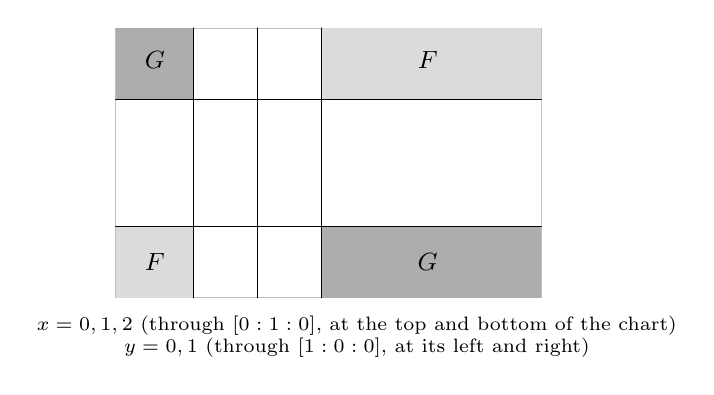
\begin{tikzpicture}[scale=0.9,line cap=round]
\draw[black!25] (-0.5,-0.4) rectangle (5.5,3.4);
\foreach \x in {0.6,1.5,2.4} \draw (\x,-0.4) -- (\x,3.4);
\foreach \y in {0.6,2.4} \draw (-0.5,\y) -- (5.5,\y);
\fill[black!14] (2.4,2.4) rectangle (5.5,3.4);
\fill[black!14] (-0.5,-0.4) rectangle (0.6,0.6);
\fill[black!32] (2.4,-0.4) rectangle (5.5,0.6);
\fill[black!32] (-0.5,2.4) rectangle (0.6,3.4);
\foreach \x in {0.6,1.5,2.4} \draw (\x,-0.4) -- (\x,3.4);
\foreach \y in {0.6,2.4} \draw (-0.5,\y) -- (5.5,\y);
\node[font=\small] at (3.9,2.95) {$F$}; \node[font=\small] at (0.05,0.1) {$F$};
\node[font=\small] at (3.9,0.1) {$G$}; \node[font=\small] at (0.05,2.95) {$G$};
\node[font=\scriptsize, align=center] at (2.9,-0.95) {$x = 0, 1, 2$ (through $[0:1:0]$, at the top and bottom of the chart)\\ $y = 0, 1$ (through $[1:0:0]$, at its left and right)};
\end{tikzpicture}
\caption{Proposition~\ref{prop:false} in the affine chart $z = 1$. Through the line at infinity, which is not in the arrangement, the two light corners form one face $F$ of $\PP$ and the two dark corners one face $G$. Their closures share no edge and meet exactly in the two centres at infinity, $[0:1:0]$ and $[1:0:0]$, two separate vertices.}\label{fig:corner}
\end{figure}

\section{The skeleton determines the arrangement}\label{sec:skeleton}

Pages~39 to~54 of folder~80 study the functor that sends a bigon-free arrangement to its \emph{decomposed skeleton}: the graph of vertices and edges, with the partition of the edges into pseudolines.

\begin{quote}
Assertion (\fac{80}, pp.~39--54). The functor from bigon-free arrangements to bigon-free decomposed skeleta is fully faithful: a bigon-free arrangement is determined by its decomposed skeleton, and every automorphism of the decomposed skeleton comes from the arrangement.
\end{quote}

The pages sketch a proof whose conditions (A1)--(A6) are said to hold ``bien entendu'', without proof. We work, as page~60 suggests, with \emph{combinatorial} arrangements: a generalised map \cite{lienhardt1994} (flags with involutions $\alpha_0, \alpha_1, \alpha_2$) of Euler characteristic $1$, whose flags are labelled by pseudolines, each pseudoline connected, passing once through each of its vertices and \emph{going straight} there (half a turn of the rotation $\alpha_2\alpha_1$ around a vertex returns to the same pseudoline), two pseudolines meeting at exactly one vertex, and every pseudoline carrying at least three vertices.

\begin{theorem}[after \fac{80}, pp.~41--54]\label{thm:skeleton}
For bigon-free combinatorial arrangements:
\begin{enumerate}
\item \emph{(Faithfulness.)} Two isomorphisms of arrangements inducing the same maps on vertices and edges are equal.
\item \emph{(Page~41, lifting.)} An isomorphism of decomposed skeleta comes from an isomorphism of arrangements iff it preserves, in both directions, the three-edge face paths (a corner continued along an edge to the next corner).
\item \emph{(Pages~42 and~50, orientation of a triangle.)} In homology modulo $2$, $\dim Z_1/B_1 \le 1$ (the relation $c_2 = c(K)$ of page~42); a pseudoline is a cycle that bounds nothing, and it crosses the boundary of any union of faces an even number of times. Consequently, for three non-concurrent pseudolines and a fourth $\Delta$ through none of their meeting points, a triangle cycle bounds iff $\Delta$ crosses an even number of its sides (condition (A5)); this is read on the skeleton and does not depend on $\Delta$.
\item \emph{(Page~54, fullness.)} If every triangle has a fourth pseudoline avoiding its three vertices, every isomorphism of decomposed skeleta lifts, uniquely, to an isomorphism of arrangements. This is the case when every triangle has a vertex on exactly two pseudolines, and in particular for simple arrangements.
\end{enumerate}
\end{theorem}

\begin{proof}[Sketch]
(1) An isomorphism of maps is determined by the image of one flag, and the flags at an edge are determined by its two vertices and the edge. (2) The face paths are the rotation system of the map (formulas (19)--(21) of the page). (3) Euler characteristic $1$ and connectedness give the dimension bound. A pseudoline, going straight, meets every other pseudoline once in half a turn around each vertex, which gives the parity statement and shows that of $z$ and $z + D$ exactly one bounds. (4) The sides of an edge are read through bounding triangles, by (3) when a fourth pseudoline avoids the triangle (conditions (A1)--(A4) at multiple points); two edges at a vertex are adjacent iff no edge lies between them; so the corners, hence the face paths, are read on the skeleton, and (2) applies. A triangle with a simple vertex always has a fourth pseudoline avoiding its vertices.
\end{proof}

\begin{figure}[ht]
\centering
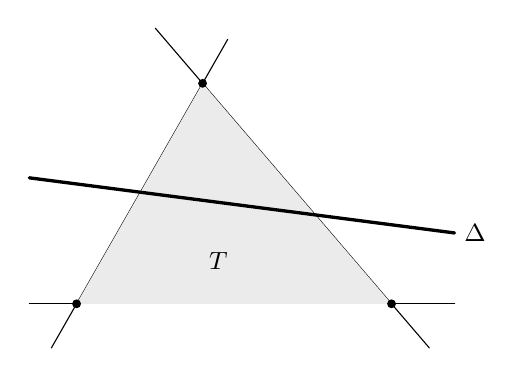
\begin{tikzpicture}[scale=1.0,line cap=round]
\coordinate (A) at (0,0); \coordinate (B) at (4,0); \coordinate (C) at (1.6,2.8);
\draw (-0.6,0) -- (4.8,0);
\draw ($(A)!-0.2!(C)$) -- ($(A)!1.2!(C)$);
\draw ($(B)!-0.2!(C)$) -- ($(B)!1.25!(C)$);
\fill[black!8] (A) -- (B) -- (C) -- cycle;
\draw[line width=1.2pt] (-0.6,1.6) -- (4.8,0.9);
\node[right,font=\small] at (4.8,0.9) {$\Delta$};
\foreach \p in {A,B,C} \fill (\p) circle (1.6pt);
\node[font=\small] at (1.8,0.55) {$T$};
\end{tikzpicture}
\caption{Condition (A5): $\Delta$ avoids the three vertices of the triangle $T$ and crosses two of its sides, an even number, so the triangle cycle bounds (the shaded face side). Had $\Delta$ crossed one side, the cycle $\partial T$ would not bound, and $\partial T + \Delta$ would.}\label{fig:A5}
\end{figure}

What remains are the triangles all of whose vertices are multiple and through which every other pseudoline passes, condition (A6) of the page; the complete quadrangle $\III$ is one of them. We reduce them to oriented matroids. A \emph{chirotope} assigns a sign to each triple of pseudolines without common point, the orientation of the triangle they form \cite{bjorner1999}.

\begin{theorem}[the edition's completion]\label{thm:chirotope}
Let $\chi$, $\chi'$ be chirotopes of two bigon-free arrangements, and $\sigma$ a bijection of the pseudolines preserving incidences, such that along every pseudoline the two cyclic orders of the vertices agree up to reversal, that is, the two chirotopes have the same separation relations along each pseudoline. Then $\chi'$ is a reorientation of $\chi$ transported by $\sigma$.
\end{theorem}

\begin{proof}[Sketch]
Along a pseudoline $i$, the other pseudolines fall into classes, one per vertex, and the sum of the signs on a cycle of four edges says whether two vertices separate two others. A sign function whose sums all vanish on a complete multipartite graph with at least three parts is a constant plus a cut. Hence the product of the two chirotopes, corrected by signs, has the form $\psi(i, j, l) = \delta^i_j\delta^i_l$ at each $i$. If a fourth pseudoline avoids a triangle, the four triples of the four pseudolines have the same value and product $1$, as in (A5). Otherwise cut the triangle $a, b, c$ along a pseudoline $x$ through $b \cap c$ and a third vertex of $a$: the triangles $a, b, x$ and $a, x, c$ each have a fourth pseudoline. In the complete quadrangle the auxiliary pseudolines are the sides through the fourth point.
\end{proof}

An isomorphism of decomposed skeleta preserves the cyclic order of the vertices along each pseudoline up to reversal, so Theorem~\ref{thm:chirotope} applies to it, and the topological representation theorem \cite{folkmanlawrence1978} turns the reorientation into a homeomorphism of $\PP$. With Theorem~\ref{thm:skeleton}(4), this gives the assertion of pages~39--54 in all cases, modulo that theorem, which is not formalised; the argument has not been read by a specialist.

\section{An added pseudoline}\label{sec:added}

Folder~154 studies the positions of a pseudoline added to an arrangement $\Sigma$. In oriented-matroid terms a position is a \emph{single-element extension} of the rank-$3$ oriented matroid of $\Sigma$, given by Las Vergnas's signature $\sigma$ on the cocircuits, the vertices of $\Sigma$, with $\sigma(-Y) = -\sigma(Y)$: the sign records on which side of the new pseudoline the vertex lies, or $0$ if on it. Las Vergnas's criterion, checked line by line, says that along each pseudoline of $\Sigma$ the signs read $+\cdots+\,(0)\,-\cdots-$ up to reversal, with at most one $0$.

Page~18 asserts that the position is determined by the cyclic order, compatible with antipody, in which the double cover of the added pseudoline meets the oriented pseudolines of $\Sigma$ (``il ne devrait pas être difficile de montrer''). In oriented-matroid terms that order is the rank-$2$ contraction at the new element.

\begin{theorem}[after \fac{154}, p.~18]\label{thm:extension}
Two single-element extensions of a rank-$3$ chirotope with the same contraction at the new element, up to a global sign, are equal, up to that sign on the triples containing the new element.
\end{theorem}

\begin{proof}
Triples not containing the new element are those of $\Sigma$. A triple containing it is, by alternation, a sign of the contraction.
\end{proof}

The proof is elementary in this form; the content of page~18 is the dictionary between pseudolines and chirotopes, again the topological representation theorem. Page~153 describes the positions near a given one $D$ through $\nu$ vertices of $\Sigma$: they correspond to the vertices of a cube of dimension $\nu$.

\begin{theorem}[Grothendieck, \fac{154}, p.~153, in oriented-matroid form]\label{thm:cube}
Let $D$ be a position, with signature $\sigma_D$ vanishing on $\nu$ vertices of $\Sigma$. A pseudoline of $\Sigma$ carries at most one vertex of $D$, and every sign vector more generic than a position, equal to it wherever it is non-zero, is a position. Consequently the positions $\sigma \ge \sigma_D$ are in bijection with all sign vectors on the $\nu$ zeros of $\sigma_D$, specialisation corresponding to specialisation: they are the faces of the cube $[-1, 1]^\nu$ ordered by reverse inclusion. There are $3^\nu$ generisations of $D$, $2^\nu$ stable ones (no zero, the vertices of the cube) and $\nu\,2^{\nu-1}$ sub-stable ones (exactly one zero, its edges).
\end{theorem}

\begin{proof}
A valid sequence $+\cdots+\,(0)\,-\cdots-$ has at most one zero, so two zeros of $D$ never lie on a common pseudoline of $\Sigma$. Replacing the zero of a valid sequence by either sign keeps it valid, and the zeros lie on different pseudolines, so the choices at the $\nu$ zeros are free and independent. The counts follow.
\end{proof}

Neither the hypothesis $\nu \ge 2$ nor the axioms of an arrangement are needed. Figure~\ref{fig:cube} shows $\nu = 2$.

\begin{figure}[ht]
\centering
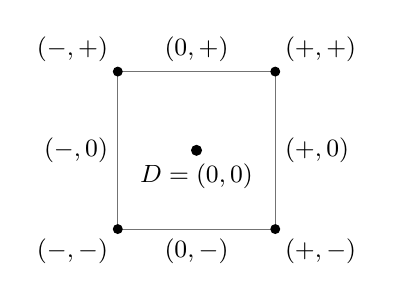
\begin{tikzpicture}[scale=1.0]
\draw[black!55] (0,0) rectangle (2,2);
\foreach \x/\y/\l in {0/0/{--\,--}, 2/0/{+\,--}, 0/2/{--\,+}, 2/2/{+\,+}} { \fill (\x,\y) circle (1.8pt); }
\node[below left,font=\small] at (0,0) {$(-,-)$}; \node[below right,font=\small] at (2,0) {$(+,-)$};
\node[above left,font=\small] at (0,2) {$(-,+)$}; \node[above right,font=\small] at (2,2) {$(+,+)$};
\node[below,font=\small] at (1,0) {$(0,-)$}; \node[above,font=\small] at (1,2) {$(0,+)$};
\node[left,font=\small] at (0,1) {$(-,0)$}; \node[right,font=\small] at (2,1) {$(+,0)$};
\fill (1,1) circle (2pt); \node[below,font=\small] at (1,0.95) {$D = (0,0)$};
\end{tikzpicture}
\caption{Theorem~\ref{thm:cube} for $\nu = 2$: the generisations of a position $D$ through two vertices, with their signs on these vertices. $D$ is the centre of the square, the $4$ stable positions its corners, the $4$ sub-stable ones its edges.}\label{fig:cube}
\end{figure}

\section{Verification}\label{sec:lean}
\begingroup\sloppy
The results above are formalised in Lean~4 with Mathlib, in \nolinkurl{Folder80Maps1.lean} (\nolinkurl{lattice_iff}, \nolinkurl{lattice_iff_not_twoPencil}, \nolinkurl{II32_not_lattice}, \nolinkurl{lattice_criterion_false}, \nolinkurl{not_lattice_of_bigonal}, \nolinkurl{not_lattice_of_four}), \nolinkurl{Folder80Maps3.lean} (\nolinkurl{faithful}, \nolinkurl{lift_iff}, \nolinkurl{finrank_Z1_le}, \nolinkurl{parity}, \nolinkurl{triangle_iff}, \nolinkurl{full_simple}, \nolinkurl{full_of_fourth'}, \nolinkurl{full_of_simpleCorner}), \nolinkurl{Folder80Signs.lean} (\nolinkurl{const_add_cut}, \nolinkurl{reorientation_of_sameSeparation}, \nolinkurl{reorientation_of_locallyEquivalent}) and \nolinkurl{Folder154.lean} (\nolinkurl{problem17_holds}, \nolinkurl{genEquiv_spec_iff}, \nolinkurl{cubeFace_subset_iff}, \nolinkurl{card_gen}, \nolinkurl{card_gen_stable}, \nolinkurl{card_gen_substable}), in the repository \href{https://github.com/Commutator-IO/grothendieck-project}{Commutator-IO/grothendieck-project}, with only Lean's standard axioms. Not formalised: the topological representation theorem of Folkman and Lawrence, hence the passage from topological pseudoline arrangements to covectors, maps and chirotopes; the surface $X^*$ of folder~154, page~150.
\endgroup

\section*{Statement on the use of artificial intelligence}
The transcriptions of folders~80 and~154, the modernised readings, the proofs, the Lean formalisation and a first draft of this text were produced with language models (Claude Opus~5 and Opus~5.5, Anthropic), under the author's direction. The author checked the statements, the proofs and the references, and takes full responsibility for the content. The formal proofs are checked mechanically by Lean.

\section*{Acknowledgements}
The facsimiles are published by the University of Montpellier, \href{https://grothendieck.umontpellier.fr/}{grothendieck.umontpellier.fr}.

\begin{thebibliography}{9}
\bibitem{bjorner1999} A.~Björner, M.~Las~Vergnas, B.~Sturmfels, N.~White, G.~M.~Ziegler, \emph{Oriented Matroids}, 2nd ed., Encyclopedia of Mathematics and its Applications~46, Cambridge University Press, 1999, \href{https://doi.org/10.1017/CBO9780511586507}{doi:10.1017/CBO9780511586507}.
\bibitem{felsnergoodman2017} S.~Felsner, J.~E.~Goodman, Pseudoline arrangements, in J.~E.~Goodman, J.~O'Rourke, C.~D.~Tóth (eds.), \emph{Handbook of Discrete and Computational Geometry}, 3rd ed., CRC Press, 2017, ch.~5.
\bibitem{folkmanlawrence1978} J.~Folkman, J.~Lawrence, Oriented matroids, \emph{J.\ Combin.\ Theory Ser.~B} 25 (1978), 199--236, \href{https://doi.org/10.1016/0095-8956(78)90039-4}{doi:10.1016/0095-8956(78)90039-4}.
\bibitem{grunbaum1972} B.~Grünbaum, \emph{Arrangements and Spreads}, CBMS Regional Conference Series in Mathematics~10, American Mathematical Society, 1972.
\bibitem{huabigon} M.~Hua, A bigon-free dichotomy for pseudoline arrangements, after a note of Grothendieck, preprint, 2026, \url{https://grothendieck.commutator.io/article/grothendieck-bigon.pdf}.
\bibitem{lienhardt1994} P.~Lienhardt, $N$-dimensional generalized combinatorial maps and cellular quasi-manifolds, \emph{Internat.\ J.\ Comput.\ Geom.\ Appl.} 4 (1994), 275--324, \href{https://doi.org/10.1142/S0218195994000173}{doi:10.1142/S0218195994000173}.
\bibitem{moharthomassen2001} B.~Mohar, C.~Thomassen, \emph{Graphs on Surfaces}, Johns Hopkins University Press, 2001.
\end{thebibliography}

\end{document}
